\begin{figure}[t]
\centering
  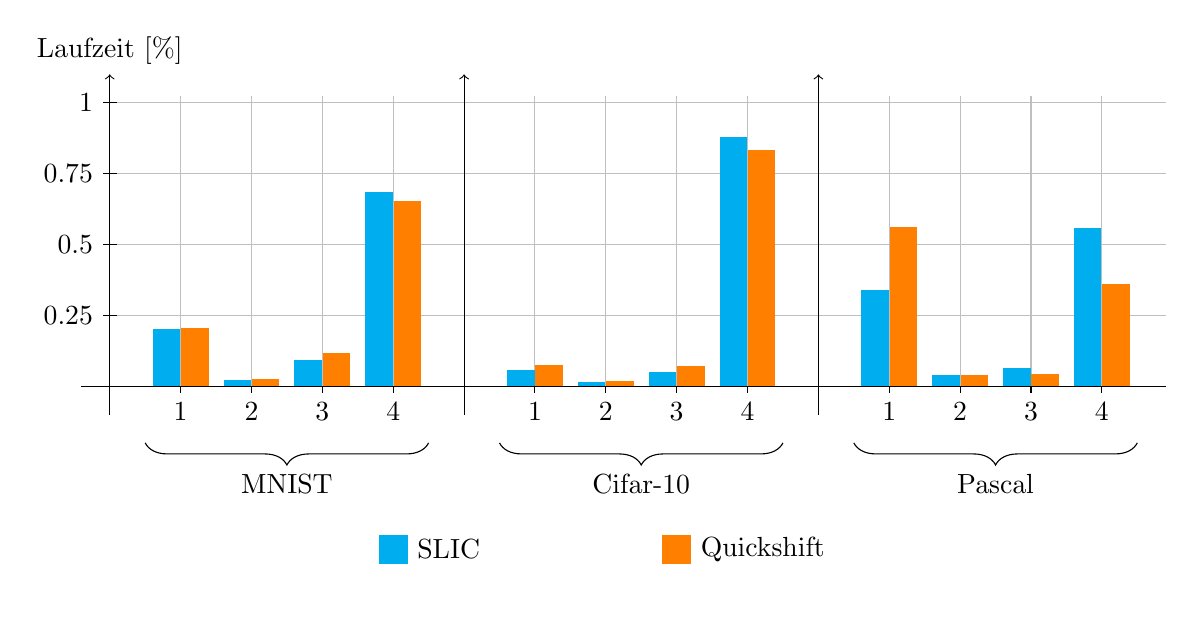
\begin{tikzpicture}[scale=0.9]
  \tikzstyle{slic}=[color=cyan, fill=cyan]
  \tikzstyle{quickshift}=[color=orange, fill=orange]

  \fill[white] (0, -2.9) rectangle (1, -1) node {};  % Abstand nach unten

  \draw[color=lightgray] (-0.1, -0.1) grid (14.9, 4.1);

  \draw[] (-0.4, 0) -- (14.9, 0);
  \draw[->] (0, -0.4) -- (0, 4.4) node[above] {Laufzeit [\%]};
  \draw[->] (5, -0.4) -- (5, 4.4);
  \draw[->] (10, -0.4) -- (10, 4.4);

  \draw (0.1, 1) -- (-0.1, 1) node[left] {$0.25$};
  \draw (0.1, 2) -- (-0.1, 2) node[left] {$0.5$};
  \draw (0.1, 3) -- (-0.1, 3) node[left] {$0.75$};
  \draw (0.1, 4) -- (-0.1, 4) node[left] {$1$};

  \draw[slic,       line width=0.35cm] (0.8, 0) -- (0.8, 4*0.2023);
  \draw[quickshift, line width=0.35cm] (1.2, 0) -- (1.2, 4*0.2054);
  \draw (1, 0) -- (1, -0.1) node[below] {$1$};

  \draw[slic,       line width=0.35cm] (1.8, 0) -- (1.8, 4*0.0212);
  \draw[quickshift, line width=0.35cm] (2.2, 0) -- (2.2, 4*0.0244);
  \draw (2, 0) -- (2, -0.1) node[below] {$2$};

  \draw[slic,       line width=0.35cm] (2.8, 0) -- (2.8, 4*0.0921);
  \draw[quickshift, line width=0.35cm] (3.2, 0) -- (3.2, 4*0.1160);
  \draw (3, 0) -- (3, -0.1) node[below] {$3$};

  \draw[slic,       line width=0.35cm] (3.8, 0) -- (3.8, 4*0.6845);
  \draw[quickshift, line width=0.35cm] (4.2, 0) -- (4.2, 4*0.6542);
  \draw (4, 0) -- (4, -0.1) node[below] {$4$};

  \draw [decoration={brace,mirror,amplitude=8pt},decorate] (0.5,-0.8) -- node[below=8pt] {\gls{MNIST}} (4.5,-0.8);

  \draw[slic,       line width=0.35cm] (5.8, 0) -- (5.8, 4*0.0568);
  \draw[quickshift, line width=0.35cm] (6.2, 0) -- (6.2, 4*0.0764);
  \draw (6, 0) -- (6, -0.1) node[below] {$1$};

  \draw[slic,       line width=0.35cm] (6.8, 0) -- (6.8, 4*0.0150);
  \draw[quickshift, line width=0.35cm] (7.2, 0) -- (7.2, 4*0.0179);
  \draw (7, 0) -- (7, -0.1) node[below] {$2$};

  \draw[slic,       line width=0.35cm] (7.8, 0) -- (7.8, 4*0.0504);
  \draw[quickshift, line width=0.35cm] (8.2, 0) -- (8.2, 4*0.0721);
  \draw (8, 0) -- (8, -0.1) node[below] {$3$};

  \draw[slic,       line width=0.35cm] (8.8, 0) -- (8.8, 4*0.8778);
  \draw[quickshift, line width=0.35cm] (9.2, 0) -- (9.2, 4*0.8336);
  \draw (9, 0) -- (9, -0.1) node[below] {$4$};

    \draw [decoration={brace,mirror,amplitude=8pt},decorate] (5.5,-0.8) -- node[below=8pt] {\gls{Cifar}-10} (9.5,-0.8);

  \draw[slic,       line width=0.35cm] (10.8, 0) -- (10.8, 4*0.3403);
  \draw[quickshift, line width=0.35cm] (11.2, 0) -- (11.2, 4*0.5601);
  \draw (11, 0) -- (11, -0.1) node[below] {$1$};

  \draw[slic,       line width=0.35cm] (11.8, 0) -- (11.8, 4*0.0385);
  \draw[quickshift, line width=0.35cm] (12.2, 0) -- (12.2, 4*0.0387);
  \draw (12, 0) -- (12, -0.1) node[below] {$2$};

  \draw[slic,       line width=0.35cm] (12.8, 0) -- (12.8, 4*0.0630);
  \draw[quickshift, line width=0.35cm] (13.2, 0) -- (13.2, 4*0.0416);
  \draw (13, 0) -- (13, -0.1) node[below] {$3$};

  \draw[slic,       line width=0.35cm] (13.8, 0) -- (13.8, 4*0.5582);
  \draw[quickshift, line width=0.35cm] (14.2, 0) -- (14.2, 4*0.3595);
  \draw (14, 0) -- (14, -0.1) node[below] {$4$};

  \draw [decoration={brace,mirror,amplitude=8pt},decorate] (10.5,-0.8) -- node[below=8pt] {\gls{Pascal}} (14.5,-0.8);

  \tikzstyle{node}=[rectangle,draw, minimum width=10pt, minimum height=10pt, inner sep=0pt]
  \node[node, slic,       label=right:\gls{SLIC}] (1) at (4, -2.3) {};
  \node[node, quickshift, label=right:Quickshift] (2) at (8, -2.3) {};
\end{tikzpicture}

\begin{tabular}{ll}
  \toprule
  1. Segmentierung & 2. Adjazenzbestimmung\\
  3. Merkmalsextraktion & 4. Receptive-Field-Berechnung\\
  \bottomrule
\end{tabular}

\caption[Laufzeitverteilung der räumlichen Vorverarbeitungsschritte]{Laufzeitverteilung der einzelnen räumlichen Vorverarbeitungsschritte für alle Datensätze und alle Superpixelalgorithmen.
Die Berechnung der Receptive-Fields umfasst je 25 Knoten bei einer Knotenauswahl mit Schrittweite $2$.
Sie zeigt sich fast in allen Datensätzen als die dominante Berechnungsaufgabe.}
\label{fig:laufzeit_raeumlich_pipeline}
\end{figure}
